\subsection{Sensitivity to the Choice of Regions (E3)}\label{sec:gdd:en:parameters}
% E3: sensitivity to the region partition.
We varied the body, transition, and tail regions used for report-driven distribution correction (Section~\ref{sec:correction}). On all four networks at $\varepsilon\in\{0.5,2\}$, we tested the quantile pairs $(0.80,0.90)$, $(0.90,0.95)$, and $(0.95,0.99)$. The middle pair is the default in E1 and E2. Each pair determines $b_1$ and $b_2$ from the base population distribution conditional on positive triangle degrees. The zero region stays fixed. 
% Vary body, transition, and tail regions using three quantile pairs; keep the zero region fixed. Reuse reports and base fits, refitting only correction strengths. Two Higgs base fits did not converge at epsilon=0.5.
The choice of regions had different effects across networks. Mean EMD varied little on Bio-DMELA and decreased at each step on DBLP at both budgets (Supplementary Material, Section~S3). Figure~\ref{fig:gdd:en:parameters} shows Higgs social and Orkut because raising both quantile levels from the lowest to the highest pair had opposite effects on these networks at $\varepsilon=0.5$. Mean EMD on Higgs social peaked at the default pair, then fell below its value at the lowest pair. On Orkut, it increased at both steps. At $\varepsilon=2$, the default gave the lowest mean EMD on Higgs social. The ordering on Orkut reversed, with mean EMD falling from 42.80 to 29.42 as the two levels increased, while both MSE and KS rose.
% Bio-DMELA EMD changes little; DBLP decreases at both budgets. Higgs and Orkut show opposite low-to-high changes at epsilon=0.5. Higgs is nonmonotone; at epsilon=2, Orkut EMD ordering reverses while MSE and KS rise.
\begin{figure}[htbp]
\centering
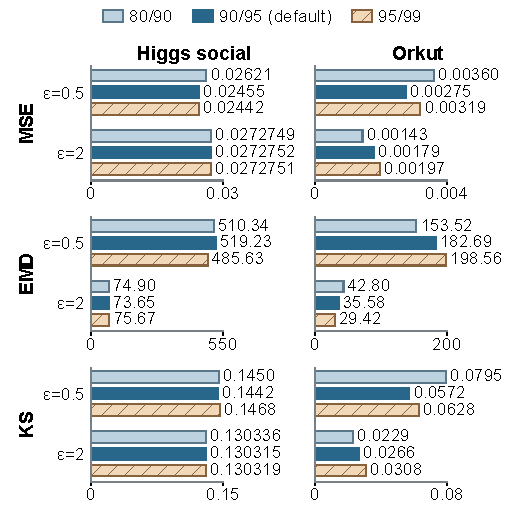
\includegraphics[width=\columnwidth]{icde_sections/figures/e3_sensitivity_means.pdf}
\caption{Sensitivity to the choice of regions on Higgs social and Orkut.}
\label{fig:gdd:en:parameters}
\end{figure}


Triangle-degree is more concentrated on Higgs social, where the top 1\% of nodes by triangle degree account for 47.6\% of the sum of triangle degrees, compared with 32.0\% on Orkut. To locate the errors at $\varepsilon=0.5$, we compared the estimates over the same percentile ranges of each network's true positive triangle-degree distribution. Moving from the lowest to the highest pair increased the EMD contribution between the 90th and 99th percentiles on both networks. On Higgs social, however, it reduced overestimation of the fraction of nodes above extreme triangle-degree thresholds. The EMD contribution above the 99.9th percentile fell in all eight paired runs, by 37.06 on average, and total mean EMD fell by 24.70. On Orkut, the same change worsened underestimation of the fraction of nodes above thresholds in the 90th--99th percentile range. The EMD contribution from this range alone rose by 43.85, close to the total increase of 45.04, and the contribution above the 99.9th percentile also rose.
% The top 1% of nodes carry a larger triangle-degree share on Higgs. Evaluation on fixed true-positive percentile ranges finds increasing 90th--99th percentile error on both networks. Reduced extreme-tail overestimation offsets other errors on Higgs; Orkut underestimation worsens. Truth is used only for evaluation.
